%
% Apunte de Sistemas Operativos
% Copyright (C) 2014 Esteban De La Fuente Rubio (esteban[at]delaf.cl)
%
% Permission is granted to copy, distribute and/or modify this document
% under the terms of the GNU Free Documentation License, Version 1.3
% or any later version published by the Free Software Foundation;
% with no Invariant Sections, no Front-Cover Texts, and no Back-Cover Texts.
% A copy of the license is included in the section entitled "GNU
% Free Documentation License".
%
% Link: http://www.gnu.org/copyleft/fdl.html
%

% MEMORIA SECUNDARIA
\chapter{Memoria secundaria}
\label{memoria_secundaria}
Durante este capítulo se abordaran temas generales relacionados con la memoria
secundaria, específicamente relacionados con el sistema de archivos y el uso del
mismo.

La memoria secundaria corresponde a aquella memoria de gran capacidad, bajo
costo pero a la vez más lenta. Una característica importante versus otros medios
de almacenamiento (como la RAM) es que corresponde a un medio persistente para
guardar datos. Estos datos serán guardados con alguna estructura dentro del
disco, la unidad mínima para trabajar con memoria secundaria, de una forma
eficiente, es el archivo.

% TODO
\begin{comment}
\section{El sistema de E/S de Unix}

API uniforma la E/S para distintos dispositivos: open, read, write y close.

FILE *f = fopen("nombre", "r");
int rc = fread(f, buf, count);

"nombre" es un archivo pero puede ser un dispositivo, ejemplos
/dev/ttyS1	puerta serial
/dev/hda1		partición de disco

La decodificación se hace por capas:

API lenguaje					fread
API núcleo						read						aplicación
---------------------------
decodificación				kread						núcleo
sistema de archivos
cache disco
scheduling disco
driver
---------------------------
disco																	hardware

La decodificación puede ser a un sistema de archivos, pero también podría ser hacia tty (y luego al driver de tty) o pipes.

Driver: presenta API genérica para los diferentes tipos de disco que puedan existir.

SATA presenta optimización al scheduling de disco, ya que por defecto se hace un poco a ciegas en la capa de scheduling de disco.

A discos ATA o PATA solo se le podía enviar un comando, en discos SATA se le pueden enviar varias peticiones y es este disco el que ejecutará el scheduling de disco en el mejor orden, básicamente para evitar mover tanto el cabezal del disco.

Las capas se podrían ver afectadas dependiendo de las capacidades que tenga el disco (como el scheduling en el mismo disco).

Discos SSD (estado solido o memoria flash) es disfrazado como un disco SATA, esto lo disfraza el driver. Tasa de transferencia mayor (300 megas, vs 50 megas de un disco tradicional) y como no hay cabezal, es mucho más rápido el acceso al disco.

Un benchmark, secuencial, da resultados 6 veces mejor en acceso (300 megas).

En acceso directo, usando lseek se leen datos del disco en puntos random del mismo. Al leer un disco tradicional el acceso aleatorio es muy MUY lento, típicamente en SSD 40 megas, en discos tradicionales es menor a 1 mega por segundo, ya que en esto hay que mover el cabezal del disco.

Controladores de discos SSD presentan diferencias entre sí, algunos pueden bajar un poco la velocidad al escribir (vs lectura), sin embargo otro controlador podría presentar una muy baja tasa de escritura.

Lo anterior es porque la memoria flash (SSD) varian mucho, ejemplos:

SDD tipo MLC, una misma celda se puede reescribir 100.00 veces (más alla podría fallar), se almacenan 2 bit por celda.

SSD tipo SLC, hasta 100.000, 1 bit por celda.

Un chip en el disco SSD reparte el uso del desgaste de los discos. En los discos SSD al escribir en el bloque 100 del disco, internamente esto se mapea a una ubicación física en el disco SSD. O sea si se escribe siempre en el bloque 100 de un disco SSD no necesariamente se escribirá en el bloque físico (real) 100 del disco SSD.

En discos tradicionales se puede sobreescribir todas las veces que uno quiera un bloque (celda) adicionalmente, si uno quiere escribir en el bloque 100 del disco repetidamente, esto se hará en el bloque 100, ya que no hay un mapeo intermedio. se escribe directamente en el bloque físico.

Para el desempeño del equipo, actualmente, es mucho más importante utilizar un disco rápido (un disco SSD) que un procesador rápido (Icore 7).

Disco tradicional duración 5 años de vida (independientemente de si esta apagada o prendido).
Seagate y western digital garantía 5 años la bajaron a 1 año.

SSD garantía de 5 años, pero tienen contadores que permiten registrar cuantas veces se ha escrito, asi que si se escribe excesivamente el fabricante lo notará y no habra garantía xD

\subsection{Decodificación}

Consideremos:

int fd = open(...);

fd (file descriptor): identifica dentro del proceso al archivo para poder comunicarse con el núcleo y poder trabajar con el archivo.

Para cada proceso hay una tabla que dice cuales son los archivos abiertos que se tienen, enumerados desde 0, donde 0 entrada estándar, 1 salida estándar y 2 salida estándar de errores.

Cada entrada de la tabla apunta a una estructura: struct file, la cual es el verdadero descriptor de archivo. Esta estructura es la que se recibe dentro del núcleo al implementar las funciones que trabajan con archivos. Dentro de esta estructura, hay diversos campos, entre ellos fops que tiene punteros hacia las implementaciones de las funciones que serán utilizadas para trabajar con el archivo (o dispositivo). Otro campo es f\_pos con la posición que se está leyendo.

read(fd, ...);

En C la decodificación (básicamente e incompleta) al hacer el read será:

\begin{verbatim}
struct file *f = tabla_fd[fd];
(*f->fops->read)(f, buf, count &f->f_pos);
\end{verbatim}

Dice incompleta porque se debe validar que el fd exista en la tabla de files descriptors.

\subsection{Sistema de archivos}

Dentro de struct file además está el campo de inodo que apunta a la tabla de inodos. El inodo apunta a una tabla que dice por cada inodo que bloques de archivo están asociados con que bloque en la partición del disco.

Inodo esta almacenado en el disco, cuando es creado o modificado el archivo, los descriptores surgen al hacer open del archivo, donde el núcleo enlaza el descriptor del archivo con el inodo.

Observación: en un fork el hijo hereda una copia de la tabla de file descriptors que tenía el proceso padre al momento de hacer el fork, ambas tablas a pesar de ser "diferentes" (iguales, pero copias) apuntarán al mismo descriptor de archivo. ¿Qué pasa si el hijo y el padre empiezan a leer el mismo archivo? Habrá problemas, ya que el file descriptor tiene la posición que se esta leyendo, y habra problema sobre dicha variable. Lo que se debe hacer es utilizar reopen (o cerrar y abrir nuevamente) para que se cree un nuevo file descritor apuntado en la tabla de files descriptors. Aunque se haga reopen, el inodo apuntado por los files descriptor (tanto padre como hijo) será el mismo (ya que esto es propio del archivo).

\subsubsection{Sistema de achivos del legado (Unix)}

Hasta ext2 era mas o menos lo del sistema del legado de Unix, no es lo que se usa pero es pedagógicamente usado.

Ext2 tenía el gra problema de journaling que es un sistema transaccional que cada vez que se graban cosas se guarda un sistema de journaling blablabla (no lo verá pq no lo conoce bien, entonces agregarlo :D)

Particiones en el disco:

              1 inodo = 128 bytes  1 bloque = 1K
------------------------------------------------
|           |                     |            |
------------------------------------------------
Superbloque  Inodos                Datos (archivos más directorios más bloques de indirección)

Super bloque 8K (por ejemplo aquí se guarda el bootloader en caso que se deje en la particion, y no en el inodo). Contiene:
- tamaño de los bloques
- número de inodos
- número de bloques
- codigo para el boot (igual que en mbr, solo el stage1 en caso de grub, ya que es un código minimó).

Los inodos representan a un archivo:
- largo, permisos, numero de usuario, numero de grupo
- número de enlaces duros
- tipo: normal (-), dispositivo (b o c), enlace simbolico (l), directorio (d)
- luego punteros para los bloques que están siendo usados en el disco.
  12 punteros a bloques en disco, si los bloques son de 1K, un archivo de 12K será manejado por un inodo. Si el archivo fuese más grande que 12K se crea un puntero de indirección simple
- puntero a indirección simple (máximo tres en el inodo), en dicho bloque no se almacenan datos, sino que se almacenan más punteros a bloques en disco, si el bloque es de 1Kbytes podrá almacenar 256 punteros de 4 bytes cada uno (32 bits para direccionar). 256 + 12 podría almacenar un archivo de 254K. Contiene punteros que van directamente a los bloques de datos.
- puntero de indirección doble : nuevamente 256 punteros, pero no a datos, sino a bloques de indirección simple. eso significa que ahora habrán 256 * 256 = 65536 bloques que se podrán direccionar de datos.
- puntero de indirección triple: apunta a 256 bloques dobles, harto espacio

tamaño máximo de archivo con bloques de 512 bytes es un poco mas de 2 GB.
Calcular con 1K, 2K y 4K

Originalmente se queria minimizar el sobrecosto en archivos pequeños, ya que originalmente los archivos eran pequeños. Para archivos mayores el sobrecosto va creciendo.

Pregunta: sobrecosto en bloques de indirección archivos de tamaño X, dar un porcentaje. Si es de 12 K sobrecosto 0, si es de 13K sobrecosto sería como 10\% ya que gastaria 1K para manejar 13K.

268KB 1K para todos esos 256 y luego... el sobrecosto menor al 0.5\% hacer calculo!!

Ventajas:
 - bajo sobrecosto en bloques de indirección
 - acceso directo eficiente, esto es la principal ventaja ya que si se quiere leer una posición X solo se debe determinar el bloque que se debe leer. El sobrecosto en el peor caso es leer tres bloques extra (triple, doble y simple) para llegar al bloque de datos, siendo esto un costo fijo.

Nota aparte: inicialmente discos eran como de 5 megas y muy caros, pcs venian sin disco

Nota: cantidad de archivos directorio raiz goku 399885, contado con
\begin{verbatim}
find / | grep -v "^/home" | wc -l
\end{verbatim}

Directorios

El inodo 0 de una partición es el directorio raíz. En caso que dicha partición no sea montada en la raiz, y sea montada en /home por ejemplo, el inodo 0 contendrá las entradas para las carpetas de /home, o sea lo usuarios.

Un directorio contiene la asociación entre nombre e inodos.

Los directorios guardan una tabla con la información para acceder a los archivos, esta información es guardada dentro del área de datos de la partición.

System V.3 la cada directorio tenia una tabla con el nombre (14bytes) y el inodo (2 bytes), donde las dos primeras filas son:
. inodo al mismo directorio
.. inodo al directorio padre

Fácil obtener el inodo de un archivo, ya que basta multiplicar por 16 la posición del archivo que se busca y obtener el inodo. Esto ya que el tamaño es fijo de los nombres.

Problema con el tamaño de nombres.

BSD 4.2 / System V.4

Cada fila tiene:
 largo del nombre (1 bytes)
 nombre (variable, máximo 256 bytes)
 inodo (2 bytes).

Nota: V3 núcleo clásico, V4 núcleo moderno (usando threads entre otras cosas)

Para marcar un archivo como borrado de un directorio se pone su largo en 0.

Si se quiere buscar el inodo de un archivo se deberá revisar todo secuencialmente, ya que no se sabe a priori en que posición está el inodo (porque el largo del nombre es variable).

Buscar un archivo:

/home/delaf/www/htdocs/index.php

Si /home es una partición:
inodo 0 de la partición /home tendrá un puntero al bloque con la tabla del directorio que tendrá la entrada delaf y el inodo del directorio /home/delaf, dicho inodo apuntara a la tabla de dicho directorio que contendra el inodo del directorio /home/delaf/www, y asi sucesivamente hasta encontrar el inodo de archivo.php

Lento la primera vez.
Rápido la segunda por el cache de disco.

¿Por qué el nombre no está en el directorio?

1. porque son de largo variable y esto implicaría que un inodo tendría que ser de 256 caractares (para el máximo posible del nombre) más los datos del inodo mencionados antes (128 bytes aproximadamente).

2. por los enlaces duros.

En un enlace duro ambos archivos apuntan al mismo inodo, entonces el nombre se guarda en los directorios y las referencias a inodo se repetira.

Ejemplo: programa /usr/bin/X11/xfig, se puede enlazar de forma dura en el directorio /usr/bin
Si xfig esta en el inodo 300 se tendrá en el directorio /usr/bin/X11 la tabla con entrada
xfig 300
luego se hace el enlace: ln /usr/bin/X11/xfig /usr/bin/xdraw
Ahora en la tabla de /usr/bin habrá una entrada:
xdraw 300
O sea con el mismo inodo :-)

Para saber cuando borrar el inodo, el campo de referencias (contador) aumentará por cada enlace duro que se cree. Inodo con numero de referencias 0, esta libre y el archivo borrado :-) Además se debe marcar en un mapa de bits (de los bloques) los bloques que ocupada ese archivo ahora como libres.

Restricción: ambos nombres tienen que estar en directorios de la misma partición. Ya que la información que se guarda es un puntero al inodo, a que inodo? al de la misma partición.

Observación: los usuarios no pueden crear enlaces duros de directorios. Por robustez no se pueden crear enlaces duros entre directorios, se podria crear un directorio que tiene referencias, pero todas esas referencias son accesibles desde el mismo no desde fuera. cueck! el resultado final de esto es un goteo de espacio en disco, ya que no se puede llegar al directorio desde fuera (a pesar de q tiene restricciones).

Ejemplo

x, contiene a y, e y contiene a z, o sea : x -> y -> z

Supongamos que en z creamos un link simbolico a y, o sea: ln y y/z/w, esto crearía una nueva entrada en los datos de z con una entrada w que apunta al inodo de y. Esto crearía un loop en el sistema. Para borrar y se requeriría borrado recursivo, pero como hay un loop esto no se podría hacer, ya que al borrar y, habria que borrar z primero, pero para borrar z hay que borrar w, pero w (que es y) con tiene a z, error!

file system check detecta estas inconsistencias, en lost+found se colocan las cosas "perdidas" que se encuentran :-)

fsck, file system check verifica y corrige la consistencia de un sistema de archivos. archivos o directorios recuperados se colocan bajo lost+found con nombres que no serán el original (ya que el nombre no está en el inodo), sino, por ejemplo, una numeración a partir de 1.

Mover un archivo

mv x y, en un archivo normal (no directorio) es igual a hacer ln x y y luego rm x.

¿Porque existe la llamada a sistema move si ya hay otras llamadas que permiten crear un enlace duro y otra para eliminar? Porque no se pueden crear enlaces de directorios, si no hubiera mv no se podrian mover (renombrar) directorios, ya que sobre directorio no se pueden usar enlaces duros.

% esto como titulo, pero no es subsubsection :-(
Gestión de bloques disponibles

I. Lista enlazada

En el superbloque va un puntero al primer bloque disponible y luego en dicho bloque un puntero al siguiente y así sucesivamente.

Francés creo ext con sistema de archivos de nombre variable (más que 14 caracteres) usando una lista enlazada. Este sistema, ext es el que se uso mucho tiempo en Unix.

En el bloque de datos, al inicio, se utiliza espacio para guardar un puntero al siguiente bloque.

Desventajas:

1. Se desordena (existe dispersión en el disco).

Bloques que se van liberando, se van colocando al inicio de la lista, por lo cual en la lista enlazada van quedando bloques apuntando a diferentes lugares en el disco, no contiguos. Al guardar un archivo que requiere 3 bloques se toman los 3 primeros apuntados por la lista, los cuales no necesariamente están contiguos.

Archivos que se crea de forma secuencial es ideal tenerlos de forma secuencial en el disco. En general los archivos se accederán de forma secuencial, hay pocas excepciones, como las bases de datos que acceden siempre de forma aleatoria (o directa).

2. Para extraer un bloque hay que leer el contenido, esto para obtener el puntero al siguiente bloque y poder actualizar el puntero inicial en el super bloque.

II. Mapa de bits (o vector de bits)

Francés se dio cuenta que no era buena idea lo de la lista enlazada y cambio el sistema de archivos para que usara un mapa de bits, esto fue ext2.

110000110110000011

Donde los 0s representan espacio disponible y los 1s espacio utilizado.

En el superbloque se guarda un mapa de bits, el cual es mantenido generalmente en la memoria del computador (sobrecosto, 0.025\% del tamaño de la partición, con bloques de 512 bytes, por lo cual podría ser menor, CALCULAR!!). También se podría mantener de forma parcial en la memoria, usando una "ventana" que da una visión de una parte del mapa de bits.

Ventajas

1. Bloques consecutivos se encuentran trivialmente.

Windows 95, 98, DOS, había problemas de "fragmentación", en realidad es dispersión. En el sistema de archivos de Unix no existe la idea de "desfragmentación" ya que con este mapa de bits, esto se evitaba.

No es mágico, si la partición esta llena, podrían haber muy pocos bloques libres y esto generaría dispersión. Esto ocurre fácilmente en discos compartidos, ya que tienen a estar llenos. Solución: Unix exige que siempre haya un 10\% de la partición disponible. A los usuarios normales se les dirá que el disco está lleno antes que realmente lo esté. Root podrá seguir creando archivos hasta llenar el disco realmente.

Desventaja general (ambos métodos de asignación)

1. Difícil recuperar un archivo que fue borrado accidentalmente, ya que si bien se pueden tener los bloques libres el orden en que esos bloques deben ser enlazados esta en los i-nodos, por lo cual si los i-nodos son reutilizados, aunque estén los datos, no se podrán recuperar.

En general:

Se prefiere journaling sobre file system check (ya que demora mucho).

\subsubsection{Sistema de archivos FAT (Microsoft Windows)}

FAT file allocation table

Para disquetes existía FAT12, esto para ahorrar al máximo el uso de bits. En ese tiempo los discos duros eran de 5 megas típicamente (en pcs de casa) por lo cual con 16 bits usando FAT16 bastaba (en ese tiempo).

HEADER   FAT   FAT' (respaldo de FAT)       Datos
---------------------------------------------------------
|       |     |                            |            |
---------------------------------------------------------

El "inodo" esta en el bloque de datos, si se corrompe un directorio, se corromperan sus datos (o sea su estructura y su contenido).

Fila en un directorio

Nombre: 8 caracteres nombre y 3 para extensión
Más datos:
Puntero al primer bloque en la fat (de 16 bits en FAT16).

Ejemplo:
Nombre: archivo.txt
Puntero: 200

Eso indica que en el bloque 200 está el primer bloque del archivo, en el bloque 200 habrá un puntero al siguiente bloque, por ejemplo 600, en el bloque 600 habrá otro puntero y así sucesivamente hasta encontrar un EOF en un puntero (en el último bloque).

Desventajas:

1. Como mucho podrán haber $2^16$ bloques como máximo en la partición. Esto significa que con bloques de 512 bytes la partición queda limitada a 32 MB.

Solución: bloques de 1K, luego de 2K, luego de 4K, etc así hasta llegar a 2GB de tamaño en la partición, el problema con esto es que los bloques eran muy grandes, por ejemplo 32KB, esto implicaba que crear un archivo de 1B ocuparía 32KB. Solución: FAT32.

2. "fragmentación" o dispersión, solución desfragmentar (pero es un proceso muy lento).

3. Nombres 8.3, solución FAT32 permite nombres largos y cortos.

Windows 98, que tenía DOS, usaba los nombres largos, pero DOS usaba nombres cortos. Ejemplo:

Nombre largo: 1234567891011.txt
Nombre corto: 123456~1.txt

Ventaja:

1. se puede recuperar archivos borrados accidentalmente muy fácilmente. Esto ya que los nombres son solo caracteres ASCII (7 bits), entonces el primer bit estaba en 0. Cuando un archivo era borrado el primer bit se colocaba en 1. Entonces el archivo no era borrado y podía ser recuperado.

% NOTA
% CDROM: variante de FAT16.
% Reproductores de música: usan FAT16 normalmente, ¿para ahorro en licencia?.
% Memorias flash y SD: usan FAT32 sin problemas... cueck...

% Nota negocio de IBM vender mainframes no PCs.

Windows lento:
- Archivo de registro disperso en el disco.
- Malware.
- Programas corriendo en background (system tray).

\subsection{Caché de disco}

Mantiene en memoria bloques recientemente leídos o escritos.

1. La primera vez que se accede se lleva del disco a la caché, futuros accesos son hechos aquí.

2. Además prelee bloques en caso de lectura secuencial (read ahead). Esto permite subir el desempeño cuando se leen varios archivos de forma secuencial en un sistema. ya que sin esto se podría comportar como acceso directo (al ser varios archivos). al usar lseek se deja de hacer read ahead.

3. Escribe bloques asincrónicamente (write after). Básicamente cuando se ocupa la llamada a sistema write, se escribe en memoria no en disco. Cada 30 segundos un demonio llama a la función sync la cual fuerza que todo lo que esté en el cache de disco a llevarlo a este. Por lo cual si uno quiere asegurarse se debe ejecutar sync. El detalle con esto es que sync envia los datos al disco, pero el disco tambien tiene un buffer, entonces después de sync esperar 1 o 2 segundos garantizará que se escriba en el disco.

Gran parte de la memoria ram del núcleo es utilizado para buffers de E/S.

\subsection{Scheduling de disco}
Solo tiene sentido en sistemas operativos multiprocesos,  no da lo mismo el orden en que se satisfacen los requerimientos. FIFO no será la mejor solución que se podría producir mucho movimiento del cabezal.

Motivación: 2 procesos compitiendo por leer archivos secuenciales en el disco. En el peor de los casos el cabezal leerá un bloque de un archivo luego un bloque del otro, esto implicará mover el cabezal, luego nuevamente se hacen los requerimientos y el cabezal se deberá mover nuevamente de un lado a otro. Esto será un problema, porque a pesar de que el archivo está secuencial en el disco (y se lee de forma secuencial) el resultado será como acceso directo.

Solución a este problema: read ahead, pero no resuelve el caso general.

Solución general: planificar el movimiendo del cabezal de tal forma que se mueva lo menor posible.

Métodos:

El sector más corto primero: se lee el sector que esté más cerca, pero esto podría provocar hambruna.

Estrategia ascensor:
Se niega a cambiar la dirección del cabezal, se mueve hacia solo un lado el cabezal. A pesar de que un nuevo requerimiento podría estar más cerca no se atenderá hasta venir de vuelta. Esto beneficiará a los sectores que estén al medio del disco.

Estrategia ascensor circular: al llegar el cabezal al final del disco parte nuevamente desde el inicio, y claro, no cambia de sentido si se hace un requerimiento más cerca en la dirección contraria.

% hasta aqui el TODO anterior (en el fondo hasta aquí era la clase de la chile)
\end{comment}

\section{Archivo}

Un \textbf{archivo} corresponderá a un conjunto de datos y/o instrucciones
relacionadas que son guardadas en un dispositivo de almacenamiento secundario,
como un disco duro o una memoria flash. Los clasificaremos en dos grupos:

\begin{itemize}
\item \textbf{Datos}: caracteres (ASCII) o binarios.
\item \textbf{Programas}: generalmente binarios, podrían ser \textit{scripts}
también.
\end{itemize}

El sistema operativo será el encargado de mapear el archivo a un conjunto de
direcciones física en el dispositivo, esto será muy similar al concepto de mapeo
de un proceso a memoria principal visto en el capítulo \ref{memoria_principal}.

\subsection{Estructura}
Un archivo deberá estar almacenado siguiendo algún formato o
\textbf{estructura}, de esta forma podremos encontrar diferentes
clasificaciones:

\begin{itemize}
	\item \textbf{Sin estructura}: solo una secuencia de bytes.
	\item \textbf{Estructura simple}: un archivo de texto con diferentes líneas, que puede ser de largo fijo o variable.
	\item \textbf{Estructura compleja}: documentos con formatos (ejemplo: pdf).
\end{itemize}

Es posible simular la estructura simple o compleja utilizando la primera, esto
definiendo caracteres de control que permiten definir el archivo. Será el
proceso que crea el archivo el que deberá decidir que estructura tendré.

Es importante mencionar que existen estructuras ya bien definidas y formatos de archivos estandarizados, por ejemplo las imágenes PNG ya tienen un formato definido, de la misma forma un gran número de archivos. En la figura \ref{fig:archivos_tipos} se pueden observar algunos de ellos, revisar /etc/mime.types para obtener una lista mayor de tipos de archivos.

\begin{figure}[htbp]
\centering
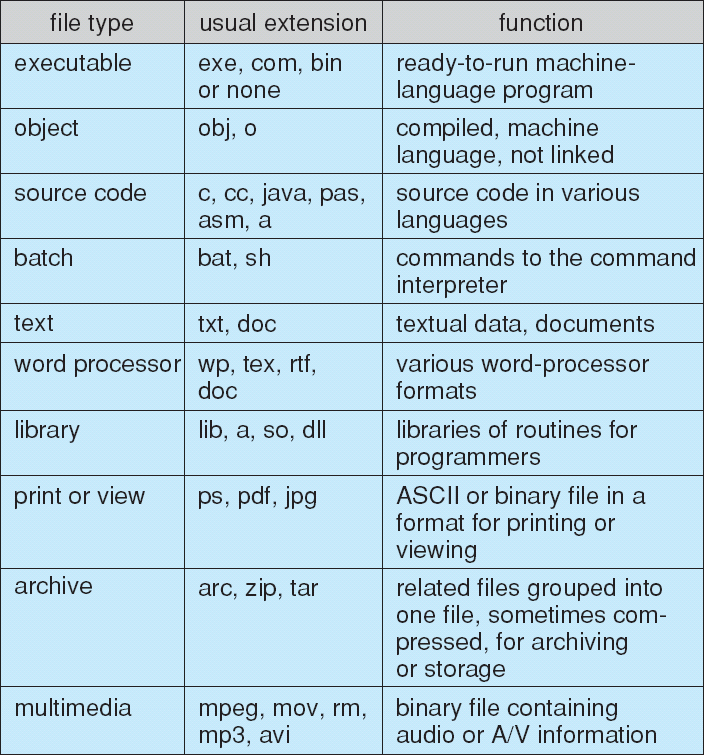
\includegraphics[scale=0.7]{img/C08_disco/tipos.png}
\caption{Diferentes tipos de archivos}
\label{fig:archivos_tipos}
\end{figure}

\subsection{Atributos}

Adicionalmente al contenido del archivo, este podrá tener diferentes
\textbf{atributos}, tales como:

\begin{itemize}
	\item \textbf{Nombre}: información en formato ``humano''.
	\item \textbf{Identificador}: etiquete (número) que lo identifica en el
sistema de archivos.
	\item \textbf{Tipo}: necesario para sistemas que soportan diferentes
tipos de archivos.
	\item \textbf{Ubicación}: puntero a la ubicación del archivo en el
dispositivo.
	\item \textbf{Tamaño}: tamaño actual del archivo.
	\item \textbf{Protección}: controla quien puede leer, escribir o
ejecutar el archivo.
	\item \textbf{Hora, fecha e identificación del usuario}: datos para
protección, seguridad y monitoreo de su uso.
\end{itemize}

A continuación se adjunta una lista con diferentes atributos de archivos
mediante la salida del comando \texttt{ls}.

% TODO quitar toda referencia a IET110 o UNAB del documento!!
\begin{verbatim}
delaf@goku:~/unab/iet110$ ls -lh
total 208K
drwxr-xr-x 3 delaf delaf 4,0K jun  4 04:00 apunte
drwxr-xr-x 3 delaf delaf 4,0K abr  9 21:01 diapos
-rw-r--r-- 1 delaf delaf  15K jun  2 15:51 iet110.ods
-rw-r--r-- 1 delaf delaf 166K nov 22  2011 IET110 Sistemas Operativos.pdf
drwxr-xr-x 5 delaf delaf 4,0K may 15 18:41 pruebas
drwxr-xr-x 5 delaf delaf 4,0K mar 25 02:38 so_juguete
drwxr-xr-x 2 delaf delaf 4,0K dic  1  2011 trabajos
-rw-r--r-- 1 delaf delaf  998 nov 22  2011 trabajo_v
\end{verbatim}

\subsection{Operaciones}

Sobre un archivo se pueden definir diversas operaciones, tales como: crear,
abrir, escribir, leer, reposicionar, eliminar, truncar o cerrar.
\texttt{Open(File)} busca en la estructura de directorios la entrada
\texttt{File} y mueve el contenido de la entrada a la memoria. De forma
contraría \texttt{Close} moverá de memoria a disco. ¿Qué sucedería si tuviese un
archivo de 100MB y solo 64MB de memoria principal?

\subsubsection{Abrir}
Para manejar un archivo abierto se requieren varias piezas de datos, estas en
conjunto permitirán traer el contenido deseado del archivo a la memoria
principal. Estas son:

\begin{itemize}
	\item \textbf{Puntero de archivo}: apunta a la última ubicación donde se
leyó o escribió el archivo, por cada uno de los procesos que tiene el archivo
abierto.
	\item \textbf{Contador de apertura}: cuenta el número de veces que el
archivo es abierto, permite remover los datos de la tabla de archivos una vez el
último proceso cierra el archivo.
	\item \textbf{Ubicación en el disco del archivo}: información para
acceder de forma física al archivo.
	\item \textbf{Permisos de acceso}: información respecto al modo de
acceso por proceso al archivo.
\end{itemize}

Algunos sistemas bloquean el acceso a los archivos si ya han sido abiertos por
otro proceso, esta es una forma de mediar con el acceso concurrente a un mismo
archivo. Cuando un archivo es abierto por primera vez el archivo es bloqueado,
luego cuando se quiere realizar una segunda apertura dos situaciones pueden
ocurrir: se puede denegar directamente el acceso al archivo o bien se puede
avisar que el archivo esta abierto y que el usuario elija que hacer, por ejemplo
abrirlo como solo lectura.

\subsection{Métodos de acceso}
Los métodos de acceso definen como se trabajara con el archivo, ya sea para
operaciones de lectura o de escritura.

\subsubsection{Acceso secuencial}
En este tipo de acceso el archivo es abierto y leído de forma continua hasta que
el archivo termina. Si se quiere leer algo nuevamente se debe volver al inicio y
empezar nuevamente.

\begin{verbatim}
/* operaciones */
read next
write next
reset
\end{verbatim}

En la figura \ref{fig:acceso_secuencial} se puede apreciar como el acceso
secuencial opera sobre un archivo. Donde desde una posición actual solo se pude
leer/escribir lo siguiente o volver al inicio.

\begin{figure}[htbp]
\centering
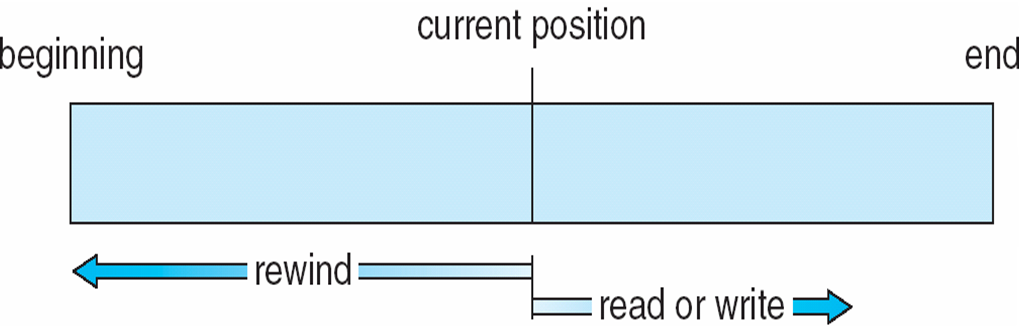
\includegraphics[scale=0.5]{img/C08_disco/acceso_secuencial.png}
\caption{Acceso secuencial a un archivo}
\label{fig:acceso_secuencial}
\end{figure}

\subsubsection{Acceso directo}
En el acceso directo se puede controlar directamente la posición del cursor
dentro del archivo, de esta forma se puede ir a una posición específica sin
tener que recorrer (leer) todo el archivo desde el inicio.

\begin{verbatim}
/* operaciones */
read n
write n
position to n
\end{verbatim}

Utilizando el acceso directo se puede simular el acceso secuencial como se ve en
la figura \ref{fig:acceso_secuencial_simulado}.

\begin{figure}[htbp]
\centering
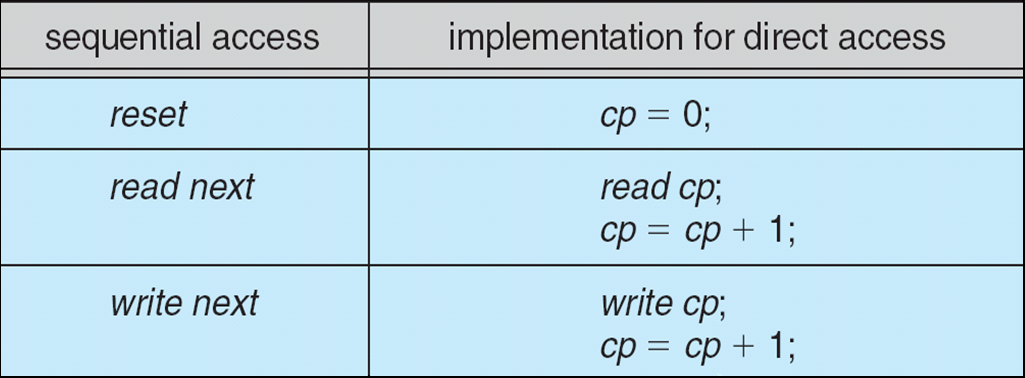
\includegraphics[scale=0.5]{img/C08_disco/acceso_secuencial_simulado.png}
\caption{Acceso secuencial simulado con acceso directo}
\label{fig:acceso_secuencial_simulado}
\end{figure}

\section{Estructura del disco}
Un disco puede ser dividido en particiones. Eventualmente estos discos o
particiones pueden ser protegidos ante fallas utilizando algún sistema, como
RAID.

Las particiones, que son las que se formatean, también son conocidas como
minidisks o slices (FreeBSD). En general la información de los discos es
guardada en una tabla de particiones, la cual permite a lo más guardar la
información de 4 particiones. Por esta razón un disco duro puede contener como
máximo 4 particiones primarias o bien 3 primarias y 1 extendida, donde la
extendida puede contener más particiones, pero lógicas.

Para utilizar el disco existen dos alternativas, escribir directamente en el
disco secuencias de bytes, en este caso se habla de un disco tipo RAW (sin un
sistema de archivo) o bien formateado con un sistema de archivos (como ext4,
reiserfs, jfs, xfs, fat, ntfs). La entidad que contiene al sistema de archivos
es conocida como un volumen, donde cada uno lleva un historial de la información
del sistema de archivos en una tabla de contenido del volumen. Así como hay
sistemas de archivos de propósito general hay aquellos que son sistemas de
archivo de propósito especial o específico, frecuentemente relacionados a un
sistema operativo

\section{Estructura de directorios}
Una estructura de directorios no es más que una colección de nodos conteniendo
información acerca de todos los archivos que contienen. Tanto la estructura de
directorio como los archivos residen en el disco, y ambas son necesarias para el
correcto funcionamiento del sistema de archivos. Por lo anterior, un respaldo
debe incluir las dos: archivos y estructura de directorios.

\subsection{Operaciones}
Sobre un directorio se pueden definir diversas operaciones, tales como: buscar
un archivo, crear un archivo, borrar un archivo, listar el contenido de un
directorio, renombrar un archivo o navegar por el sistema de archivos.

\subsection{Organización de los directorios}
El objetivo de dar una organización, orden o jerarquía a los directorios tiene
relación con:

\begin{itemize}
	\item \textbf{Eficiencia}: poder ubicar un archivo rápidamente.
	\item \textbf{Nombres}: dos o más usuarios podrían tener el mismo nombre
para diferentes archivos o bien el mismo archivo tener diferentes nombres.
	\item \textbf{Agrupar}: agrupar los archivos por propiedades, usos o
tipos (ej: binarios, configuraciones, datos variables, etc).
\end{itemize}

\subsubsection{Nivel simple}
En este caso solo existe un nivel de directorios, ver figura
\ref{fig:jerarquia_nivel_simple}. Aquí los mayores problemas son los nombres de
los archivos y la baja capacidad de agrupamiento.

\begin{figure}[htbp]
\centering
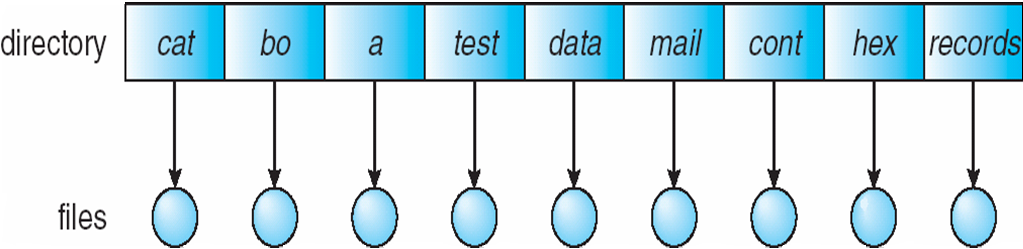
\includegraphics[scale=0.5]{img/C08_disco/jerarquia_nivel_simple.png}
\caption{Jerarquía de directorios simple}
\label{fig:jerarquia_nivel_simple}
\end{figure}

\subsubsection{Dos niveles}
En este caso se definen directorios separados para cada usuario, ver figura
\ref{fig:jerarquia_dos_niveles}. Esto permite tener el mismo nombre de archivo
para diferentes usuarios y provee de una búsqueda eficiente. Sin embargo las
capacidades de agrupar son muy limitadas.

\begin{figure}[htbp]
\centering
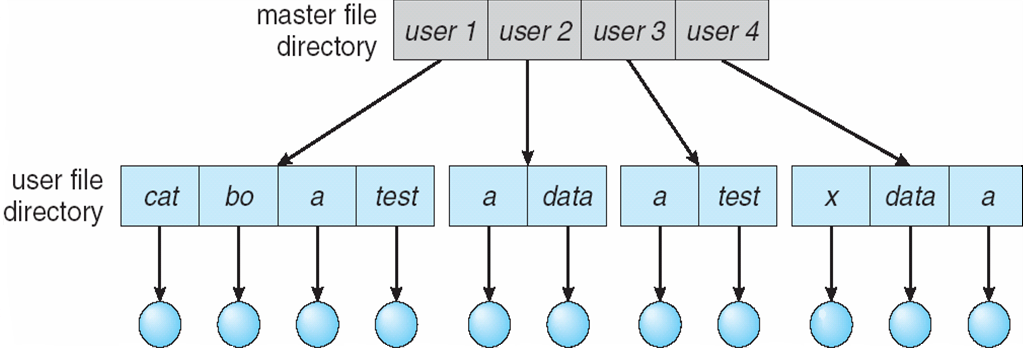
\includegraphics[scale=0.5]{img/C08_disco/jerarquia_dos_niveles.png}
\caption{Jerarquía de directorios con dos niveles}
\label{fig:jerarquia_dos_niveles}
\end{figure}

\subsubsection{Jerarquía en árbol}
En este tipo se crean ``infinitos'' niveles de subdirectorios, tantos como sean
necesarios, ver figura \ref{fig:jerarquia_arbol}. Provee de una búsqueda
eficiente, permite tener nombres de archivos repetidos y permite entregar
capacidades de agrupamiento.

\begin{figure}[htbp]
\centering
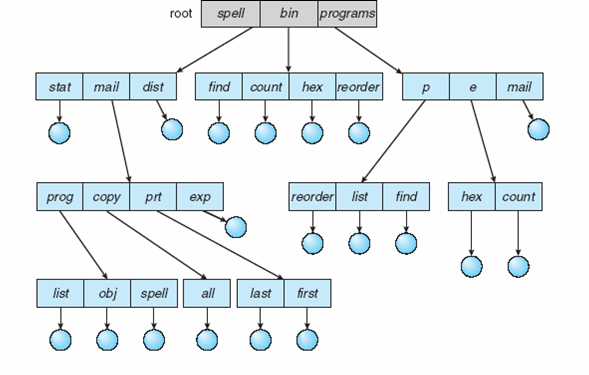
\includegraphics[scale=0.8]{img/C08_disco/jerarquia_arbol.png}
\caption{Jerarquía de directorios en árbol}
\label{fig:jerarquia_arbol}
\end{figure}

En este tipo de estructura de definen dos formas de navegar por el árbol de
directorios, mediante \textbf{rutas absolutas} que parten desde la raíz del
árbol o mediante \textbf{rutas relativas} que parten desde donde uno se
encuentra ``parado'' en el árbol.

Respecto al borrado de archivos o directorios, esta debe ser realizada de forma
recursiva, ya que se deben ir quitando las referencias entre directorios y
archivos de tal forma de no dejar nodos o hojas sin un nodo padre.

\section{Montaje}
Un sistema de archivos debe ser montado antes de poder ser accedido. Este
proceso se lleva acabo ``tomando'' el volumen no montado y ``ubicándolo'' en un
punto de montaje. Este punto de montaje corresponderá a algún directorio dentro
del sistema de archivos.

Si se llega a montar un volumen sobre un directorio que ya contiene archivos u
otros directorios estos no se perderán, solo quedarán inaccesibles hasta que el
volumen sea desmontado.

\section{Compartición}
Para compartir un archivo (o directorio) dentro del árbol de directorio se
pueden utilizar \textit{aliases} para nombrar a un mismo elemento en diferentes
partes del árbol.

En la figura \ref{fig:archivos_enlaces} se puede apreciar la compartición donde
un mismo archivo se encuentra en dos carpetas \texttt{count} y de forma similar
dos carpetas \texttt{w} y \texttt{words} apuntan a una misma llamada
\texttt{list}.

\begin{figure}[htbp]
\centering
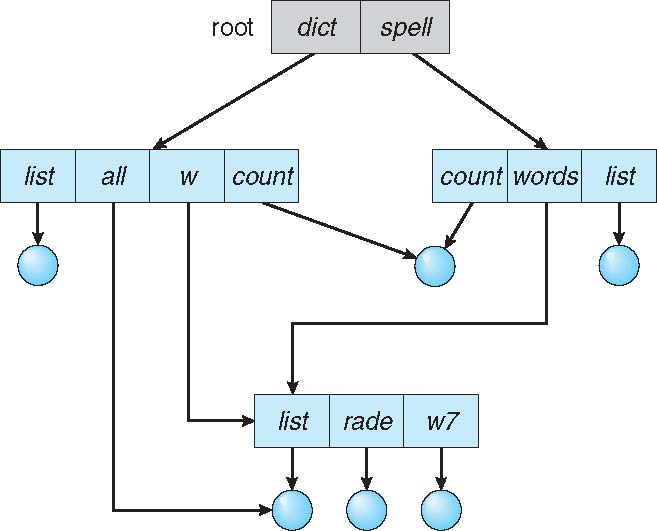
\includegraphics[scale=1]{img/C08_disco/enlaces.jpg}
\caption{Enlaces}
\label{fig:archivos_enlaces}
\end{figure}

Lo anterior es conocido como un enlace, lo cual será otro nombre (un puntero) a un archivo ya existente. Cuando se quiera acceder al enlace se deberá resolver siguiendo el puntero para localizar el archivo. Se definen dos tipos de enlaces:

\begin{enumerate}[i.]
	\item Enlaces simbólicos:
	\begin{itemize}
		\item Tamaño del enlace, tamaño de la ruta hacia el archivo.
		\item Apunta a una ruta en el sistema de archivos.
		\item Puede ser utilizado entre diferentes sistemas de archivos.
	\end{itemize}
	\item Enlaces duros
	\begin{itemize}
		\item Apunta al dispositivo de almacenamiento.
		\item Tamaño del enlace, tamaño del archivo.
		\item Solo puede ser utilizado en un mismo sistema de archivo.
	\end{itemize}
\end{enumerate}

\subsection{Protección}

Compartir archivos en un sistema multiusuarios es una tarea deseable, pero se debe considerar un esquema de protección para evitar que cualquier usuario pueda realizar cualquier tipo de operación sobre los archivos.

El propietario del archivo debe ser capaz de controlar ¿qué puede ser hecho? y ¿por quién puede ser hecho?. Para esto se utiliza el identificador del usuario (UID) y de grupo (GID) permitiendo definir los permisos que disponen cada uno de los usuarios del sistema sobre los archivos y directorios. Se definen tres tipos básicos de permisos: lectura (read), escritura (write) y ejecución (execute)

A continuación se explica la salida del comando \texttt{ls -l} que involucra los permisos recién descritos:

\begin{verbatim}
-rw-r--r--  1 usuario grupo    289 nov 20 23:08 archivo
- -  -  -   -                   -   -
| |  |  |   |                   |   |
| |  |  |   |                   |   +----- fecha de modificación
| |  |  |   |                   +--------- tamaño
| |  |  |   +----------------------------- enlaces duros
| |  |  +--------------------------------- permisos otros
| |  +------------------------------------ permisos grupo
| +--------------------------------------- permisos usuario
+----------------------------------------- tipo (común '–' o 'd')
\end{verbatim}


\section{Ejercicios y preguntas}
\begin{enumerate}
	\item Nombre 5 atributos de un archivo.
	\item Explique las partes involucradas en la apertura de un archivo.
	\item ¿Cuál es la diferencia entre el método de acceso secuencial y directo hacia un archivo?.
	\item ¿Se puede simular el acceso secuencial a un archivo con acceso directo?, explique.
	\item ¿Se puede simular el acceso directo a un archivo con acceso secuencial?, explique.
	\item ¿Cuántas particiones primarias se pueden crear en un disco? ¿por qué?.
	\item ¿Qué implica usar un disco como RAW?.
	\item ¿Cuales son los objetivos de la organización del disco?.
	\item ¿Por qué la estructura jerárquica simple no cumple con los objetivos?.
	\item ¿Cuál es la diferencia entre rutas relativas y rutas absolutas?.
	\item ¿Qué es el proceso de montaje?.
	\item ¿Cuál es la diferencia entre enlaces simbólicos y duros?.
	\item ¿Cuáles son los tres permisos definidos para un archivo o directorio?.
\end{enumerate}

\section{Referencias}
\begin{itemize}
	\item Sistemas Operativos, Segunda Edición, Andrew Tanenbaum, Capítulo 5.
	\item Sistemas Operativos, Quinta Edición, Abraham Silberschatz y Peter Baer Galvin, Capítulo 10 y 11.
	\item Sistemas Operativos, Segunda Edición, William Stallings, Capítulo 10 y 11.
\end{itemize}
